\href{../README.md}{\textless--}

\begin{center}\rule{0.5\linewidth}{0.5pt}\end{center}

\section{Cours 12}\label{cours-12}

\subsection{Rappels}\label{rappels}

Le \emph{système de fichier} est une interface \emph{unifiée} et unique
des différents périphériques de stockage (car bcp de type différent). On
a une hiérarchie en \textbf{point de montage} (\texttt{mnt})

On a une grande diversité des supports: 1. Les Disques Durs avec des
têtes de lectures basé sur les champs électro-magnétique

\begin{figure}
\centering
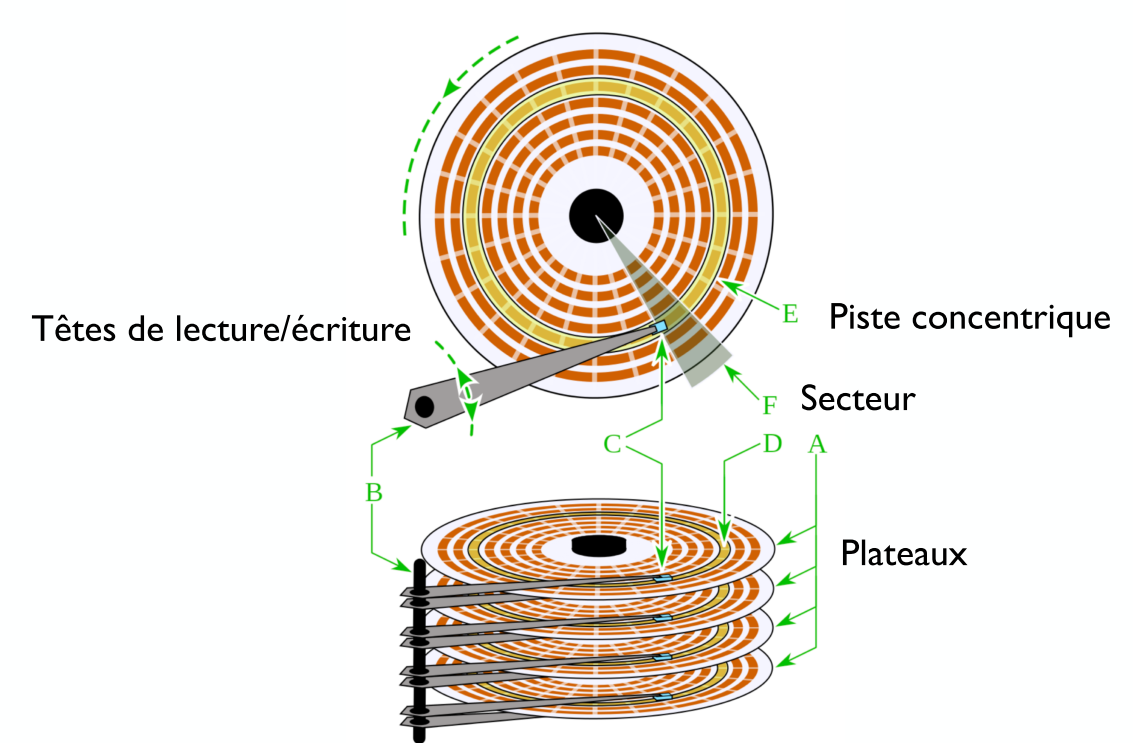
\includegraphics{image-35.png}
\caption{Alt text}
\end{figure}

\begin{enumerate}
\def\labelenumi{\arabic{enumi}.}
\setcounter{enumi}{1}
\tightlist
\item
  SSD: plus compliqué avec du flash, de la RAM buffer, \ldots{}
\end{enumerate}

\begin{figure}
\centering
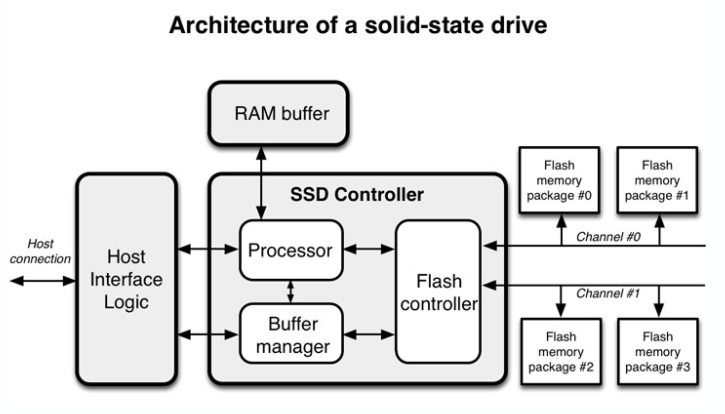
\includegraphics{image-36.png}
\caption{Alt text}
\end{figure}

\subsection{Abstraction du Matériel}\label{abstraction-du-matuxe9riel}

On a néanmoins une abstraction du matériel à faire pour que tout
fonctionne de manière uniforme:

\begin{figure}
\centering
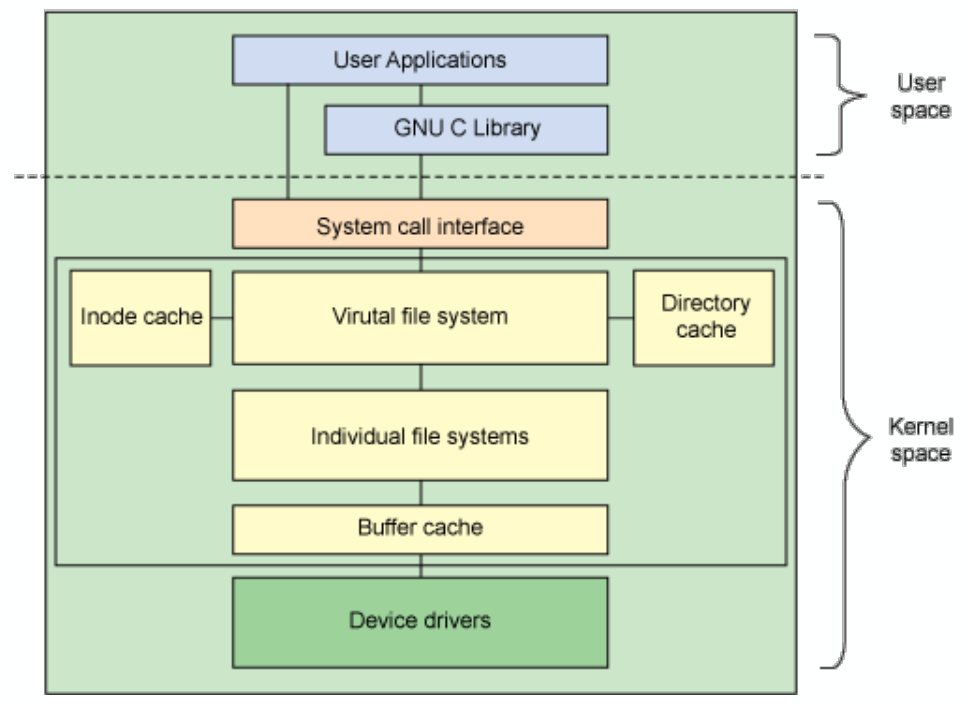
\includegraphics{image-37.png}
\caption{Alt text}
\end{figure}

Le fait qu'un dispositif de stockage utilise des plateaux, ram, \ldots{}
est géré via les \emph{devices drivers} et le \emph{gestionnaire de
périphérique} (interface logiciel kernel/matériel).

Comme précédemment, on va gérer le stockage via des blocs de
\texttt{4\ Ko} (même taille qu'un page mémoire wow). On peut tout de
même avoir une \textbf{granularité} différente (typiquement:
\texttt{512} octets pour un HDD et entre \texttt{256} et \texttt{4096}
octets pour un SSD).

\subsubsection{Les partitions}\label{les-partitions}

C'est le faite de virtuellement segmenter un support de stockage en
multiples morceaux.

On va retrouver au début des disques des
\textbf{\texttt{boot\ control\ block}} et dans chaque début de
\textbf{partitions} des \textbf{\texttt{partition\ control\ block}}.

\begin{figure}
\centering
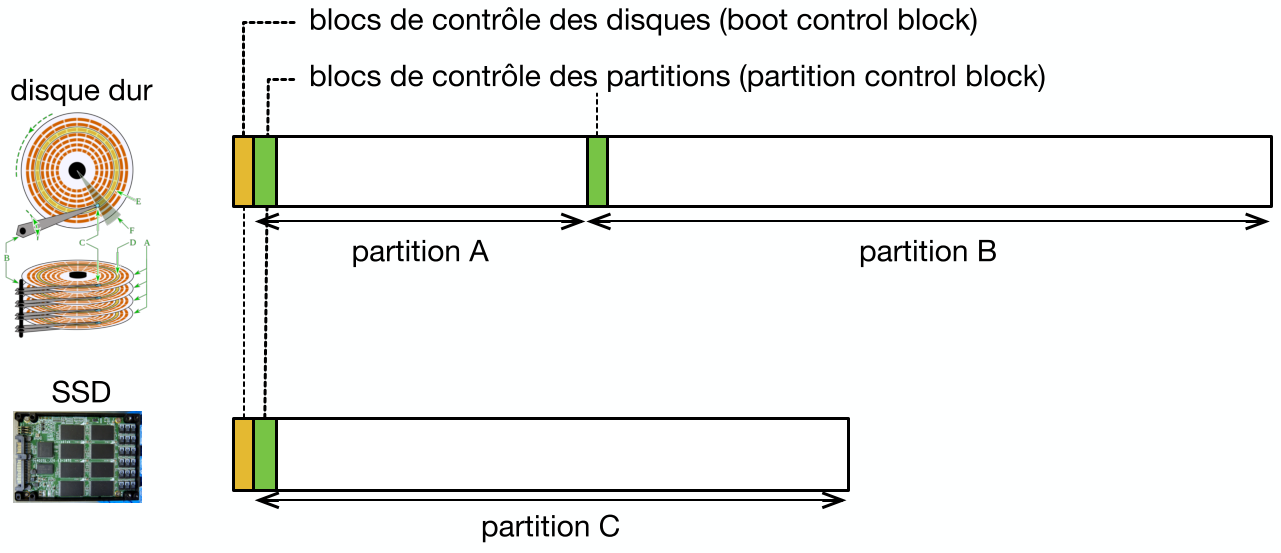
\includegraphics{image-39.png}
\caption{Alt text}
\end{figure}

\paragraph{\texorpdfstring{\texttt{boot\ control\ block}}{boot control block}}\label{boot-control-block}

C'est là où est stocké le GRUB, c'est la première chose lue au démarrage
! (\emph{cela contient des programmes de bootstrap}).

Il contient aussi des infos sur la taille des partitions et sur les
\textbf{secteurs défectueux}.

\paragraph{\texorpdfstring{\texttt{partition\ control\ block}}{partition control block}}\label{partition-control-block}

Dépend du système d'exploitation (NTFS, FAT32, \ldots). On a des infos
utiles pour monter la partition. C'est le point de démarrage pour
structurer un \emph{système de fichier}.

Cela indique aussi si on a un démontage propre la dernière fois
(\emph{oui oui éjecter la clé USB là}).

\paragraph{\texorpdfstring{Partition de
\texttt{swap}}{Partition de swap}}\label{partition-de-swap}

C'est là où on voit les \emph{pages évincés par la mémoire virtuelle}
(cf: cours 10).

On crée une telle partition via \texttt{mkswap} et on l'active via
\texttt{swapon}.

C'est simplement un bloc de métadonnées et le reste est utilisé comme
\emph{cadre de page}. Les données ne doivent pas être persistante.

\section{Structure d'un Système de
Fichier}\label{structure-dun-systuxe8me-de-fichier}

Généralement on a des blocs de \texttt{4\ Ko}. Donc un fichier occupe
toujours un nombre entier de bloc (\texttt{100\ o} fichier
--\textgreater{} \texttt{4\ Ko} sur disque). Donc on perd généralement
de l'espace dans le dernier bloc.

On veut donc savoir quels blocs sont libres ou occupés, c'est un peu le
même problème qu'avec \texttt{malloc}.

\subsection{Stockage et Allocation des
Blocs}\label{stockage-et-allocation-des-blocs}

Donc après les différents blocs de contrôle, on va avoir une
\textbf{table d'allocation}. La table est indexée par le \emph{numéro du
fichier}.

Chaque entrée contient les métadonnées (permission, propriétaire,
\ldots) et permet d'accéder à la liste des blocs donnés.

\begin{figure}
\centering
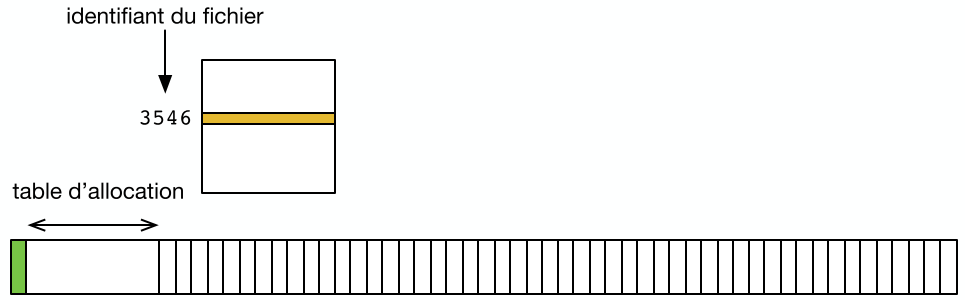
\includegraphics{image-40.png}
\caption{Alt text}
\end{figure}

Mais on doit s'intéresser à comment stocker un fichier et si sa taille
venait à changer.

\subsubsection{Option 1}\label{option-1}

On écrit simplement les blocs les un à la suite de l'autre et on stocke
simplement le pointeur vers l'entrée du premier blocs.

\begin{figure}
\centering
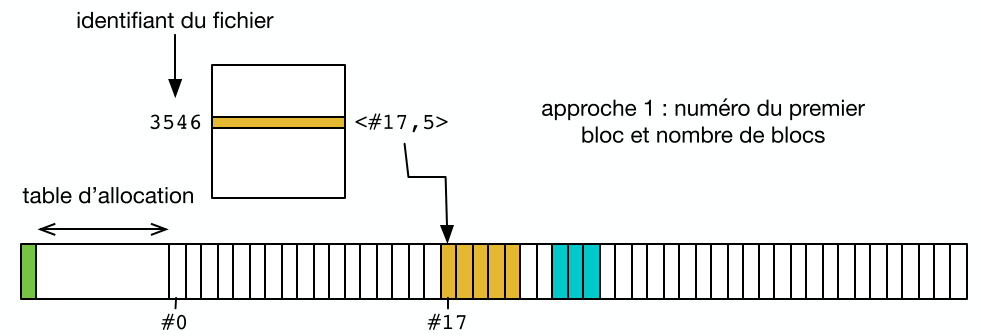
\includegraphics{image-41.png}
\caption{Alt text}
\end{figure}

\begin{itemize}
\tightlist
\item[$\boxtimes$]
  Simple
\item[$\square$]
  Compliqué d'agrandir un fichier
\item[$\square$]
  Fragmentation --\textgreater{} on a plein de blocs vides entre les
  blocs alloués
\end{itemize}

\subsubsection{Option 2}\label{option-2}

On stocke l'entrée pour le premier bloc puis on fait des pointeurs vers
le suivant etc etc ou avec un \texttt{EOF} (End Of File) si plus rien.

\begin{figure}
\centering
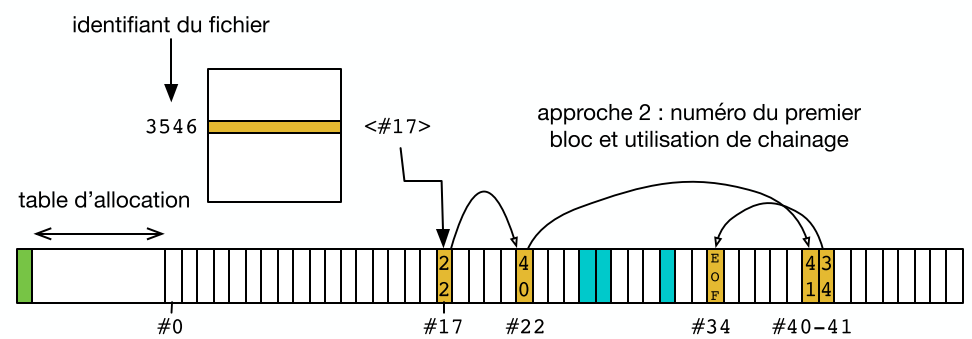
\includegraphics{image-42.png}
\caption{Alt text}
\end{figure}

\begin{itemize}
\tightlist
\item[$\boxtimes$]
  N'empêche pas de réserver tout l'espace libre
\item[$\square$]
  Localité HORRIBLE (le pire c'est sur un HDD)
\item[$\square$]
  On doit parcourir le fichier pour accéder au milieu
\end{itemize}

\subsubsection{FAT32}\label{fat32}

Pour \textbf{File Allocation Table} utilisé sur MS-DOS et Windows
(standard sur clé USB).

\paragraph{Combine 2 approches}\label{combine-2-approches}

On a une allocation des blocs \emph{contiguës} et liste chainé entre
\emph{groupe de blocs}. Croissance possible sans déplacement de blocs.

\begin{itemize}
\tightlist
\item[$\boxtimes$]
  Simple
\item[$\square$]
  Grande fragmentation et perte de la localité avec le temps
\end{itemize}

\paragraph{(Dé)Fragmentation}\label{duxe9fragmentation}

Une solution à ce problème est de \textbf{défragmenter} son disque.

Très important sur HDD, pas nécessaire sur Linux via \texttt{ext4} qui
prend des mesures en amont.

\subsubsection{Stockage indexé}\label{stockage-indexuxe9}

On ne va plus utiliser une table de en début de partition mais on va
utiliser certains blocs (\textbf{bloc d'index}) pour stocker les
métadonnées.

\begin{figure}
\centering
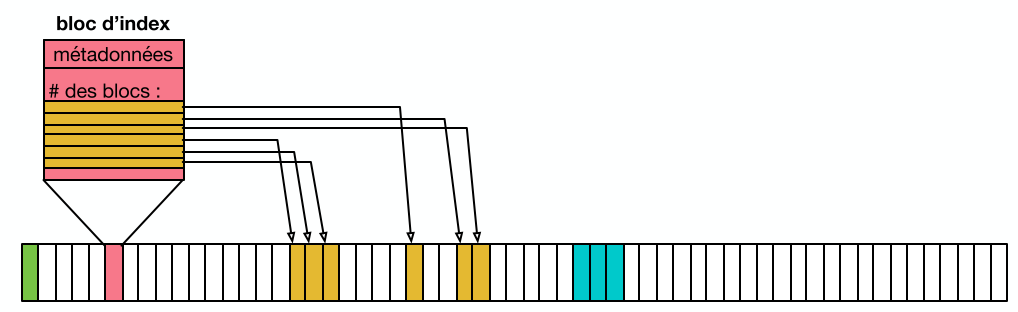
\includegraphics{image-43.png}
\caption{Alt text}
\end{figure}

\begin{itemize}
\tightlist
\item[$\boxtimes$]
  Pas de limitation à l'avance du nombre de fichiers.
\item[$\square$]
  On a besoin de 1 bloc en plus même pour des petits fichiers.
\end{itemize}

On peut utiliser tout l'espace mais on fait face à un risque
d'\emph{éparpillement}.

La taille du fichier est limité par la taille du bloc d'index.
--\textgreater{} si on a \texttt{4\ Ko} avec \texttt{4\ o} par entrée
cela signifie qu'on peut avoir que \texttt{800} entrées donc la taille
maximum est de \texttt{4\ Ko\ x\ 800} \textasciitilde{} \texttt{3\ Mo}.

\subsubsection{\texorpdfstring{Système de Fichiers
\texttt{ext4}}{Système de Fichiers ext4}}\label{systuxe8me-de-fichiers-ext4}

C'est le système de fichier standard et très généraliste et opti.

Mélange entre table d'allocation et blocs d'index. On a des
\emph{inodes} qui contient des métadonées et liens vers les blocs de
contenu.

Les inodes peuvent être inférieures à \texttt{4\ Ko}. Cela favorise la
localité des informations.

\begin{figure}
\centering
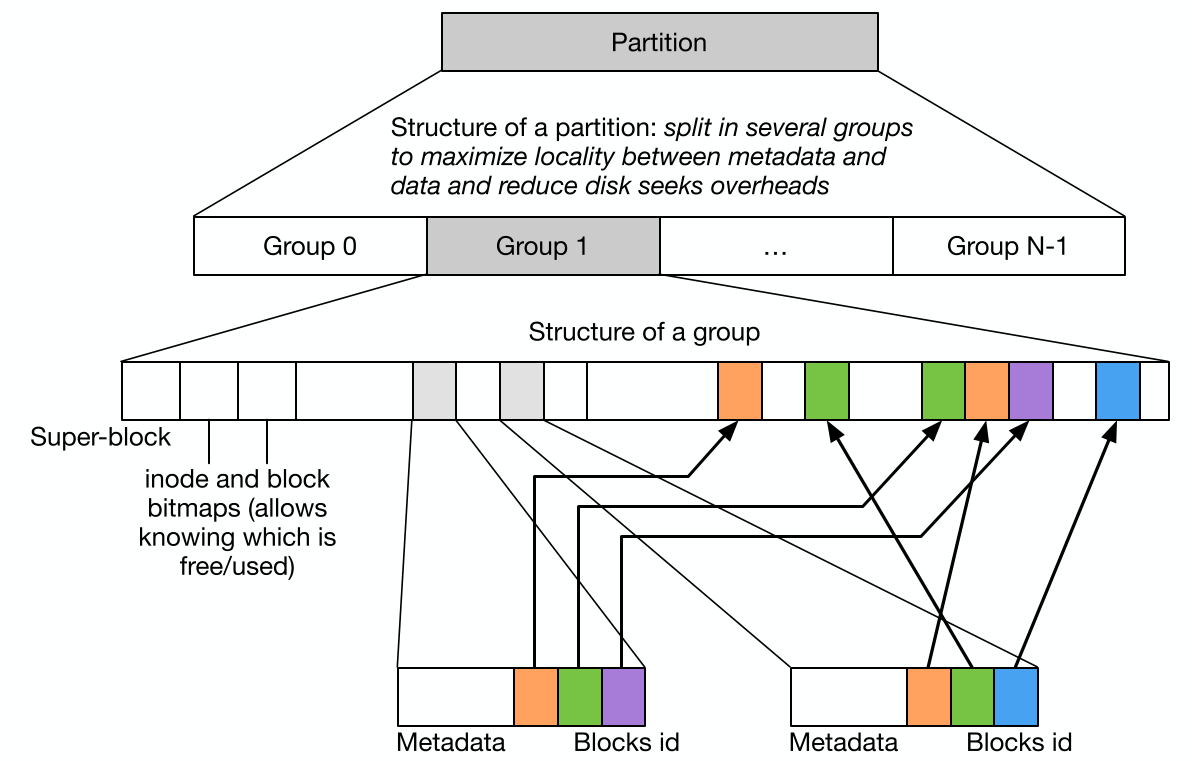
\includegraphics{image-44.png}
\caption{Alt text}
\end{figure}

L'idée c'est de faire des arbres d'inodes, donc on peut avoir des arbres
triples, doubles, simples , \ldots{}

\begin{figure}
\centering
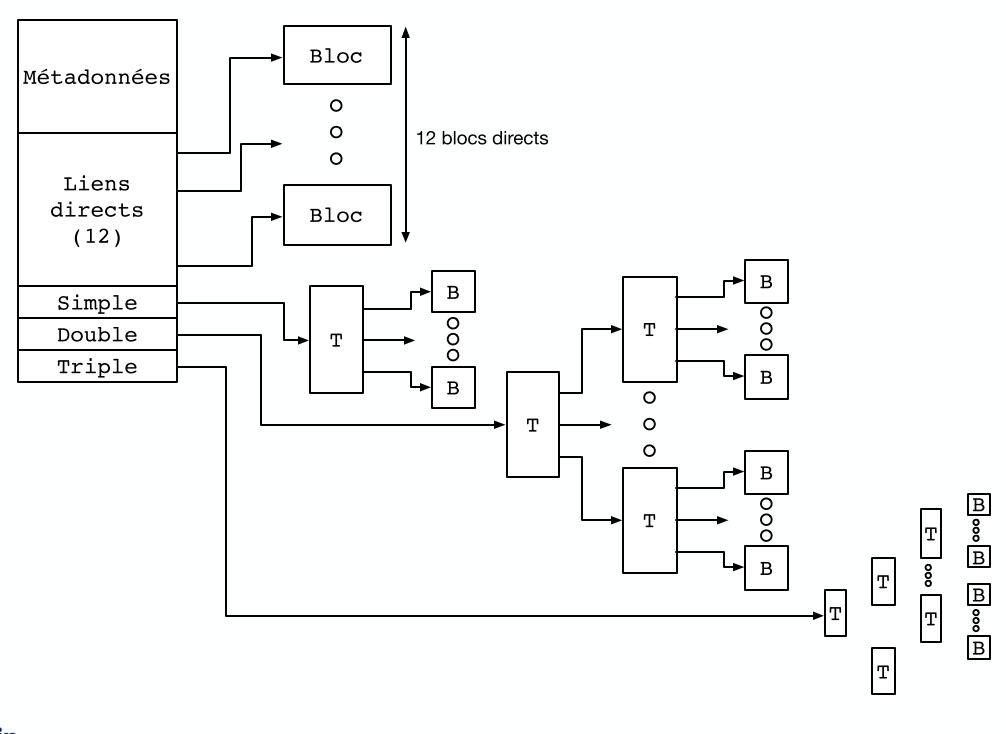
\includegraphics{image-45.png}
\caption{Alt text}
\end{figure}

\subsection{Stockage des Répertoires}\label{stockage-des-ruxe9pertoires}

Un répertoire est stocké comme un fichier. On va juste indiquer qu'il
s'agit d'un répertoire via des métadonnées via un bit \texttt{d}. On y
liste aussi les blocs de données (peut utiliser plusieurs blocs de
données).

Via \texttt{ext4}, stockage de petite liste de fichiers directement dans
l'inode.

\subsection{Gestion de l'Espace Libre}\label{gestion-de-lespace-libre}

On a une liste qui indique les blocs libres sur le disque qui est
conservé avec le temps.

\subsubsection{Effacer un Fichier}\label{effacer-un-fichier}

\texttt{rm} va juste supprimer l'entrée dans le répertoire et mettre
dans celle des blocs libres si plus aucun lien ne pointe vers ce
fichier.

L'inode et le bloc \textbf{ne sont pas effacés}. (donc on peut récupérer
des données même si elles ont été ``\emph{effacées}'')

\subsubsection{Performance et Cache}\label{performance-et-cache}

Un SSD est 1000 fois plus lent que de la RAM et un HDD est 1000000 de
fois plus lent. On va donc utiliser du cache.

\begin{figure}
\centering
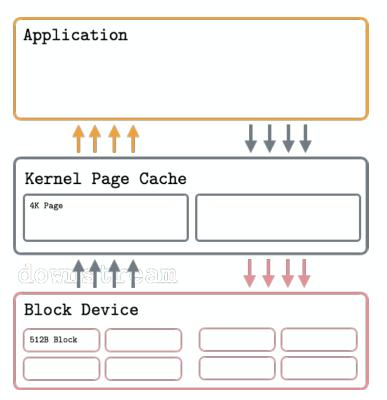
\includegraphics{image-46.png}
\caption{Alt text}
\end{figure}

Le cache se situe au niveau du \textbf{contrôleur de périphérique et/ou
du disque}.

On peut utiliser la mémoire comme cache pour les accès disque. On peut
faire cela via la mémoire virtuelle et \texttt{mmap}.

\subsection{Optimisations}\label{optimisations}

\paragraph{Disque Dur}\label{disque-dur}

On va éviter de faire trop bouger la tête de lecture, donc on écrit sur
la partie la plus extérieure du disque.

On a un accès souvent séquentiel aux fichiers donc pas de retour en
arrière, on lit tout d'une traite: - \emph{read-ahead}: on charge les
blocs suivants - \emph{read-behind}: on libère les pages du cache au fur
et à mesure.

\begin{figure}
\centering
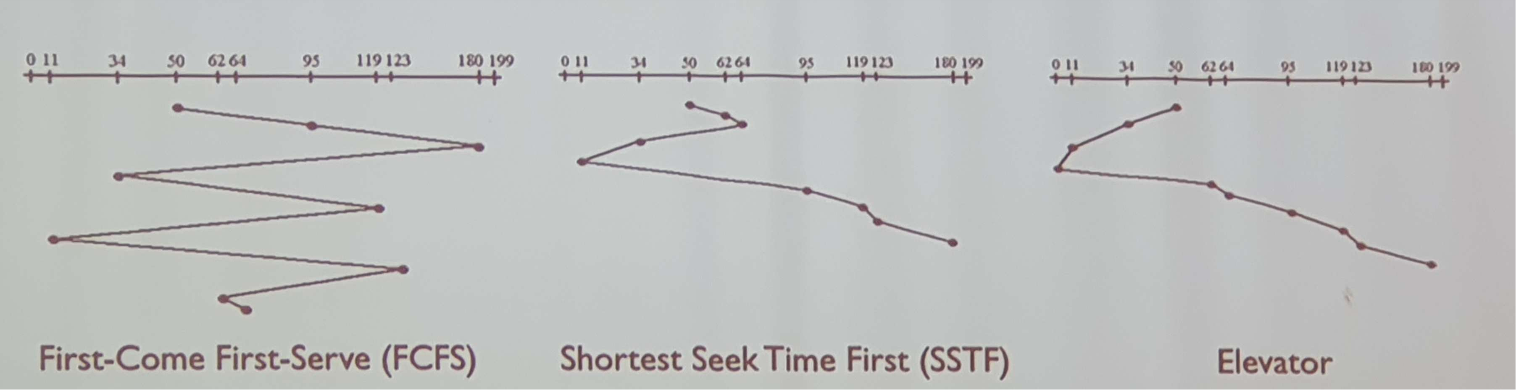
\includegraphics{Drawboard-PDF-Annotation-Copy.png}
\caption{Alt text}
\end{figure}

On va éviter les approches FIFO et privilégier soit une approche SSTF où
on se déplace du moins possible ou changer de direction le moins
possible via un algorithme de l'ascenseur.

\subsubsection{Robustesse}\label{robustesse}

Il faut que les données du disque restent cohérente malgré les mauvais
démontage, \ldots{}

On va donc avoir de la redondance et des vérificateurs de fichiers. On
peut vérifier que la liste des blocs vides ne pointent pas vers un bloc
listé par une inode.

\paragraph{Journalisation}\label{journalisation}

TODO

\begin{center}\rule{0.5\linewidth}{0.5pt}\end{center}

\href{../README.md}{\textless--}
